\documentclass[tikz,border=3pt]{standalone}

\usetikzlibrary{positioning,arrows.meta,calc,fit,backgrounds}
\definecolor{ink}{HTML}{0B0B0B}
\definecolor{ink2}{HTML}{52514E}
\definecolor{adj}{HTML}{2A78D6}
\definecolor{adjl}{HTML}{CDE2FB}
\definecolor{pinn}{HTML}{EB6834}
\definecolor{pinnl}{HTML}{FBDCCC}
\definecolor{joint}{HTML}{14855C}
\definecolor{jointl}{HTML}{CDEFE2}
\definecolor{neut}{HTML}{F1F0EC}
\begin{document}
\sffamily
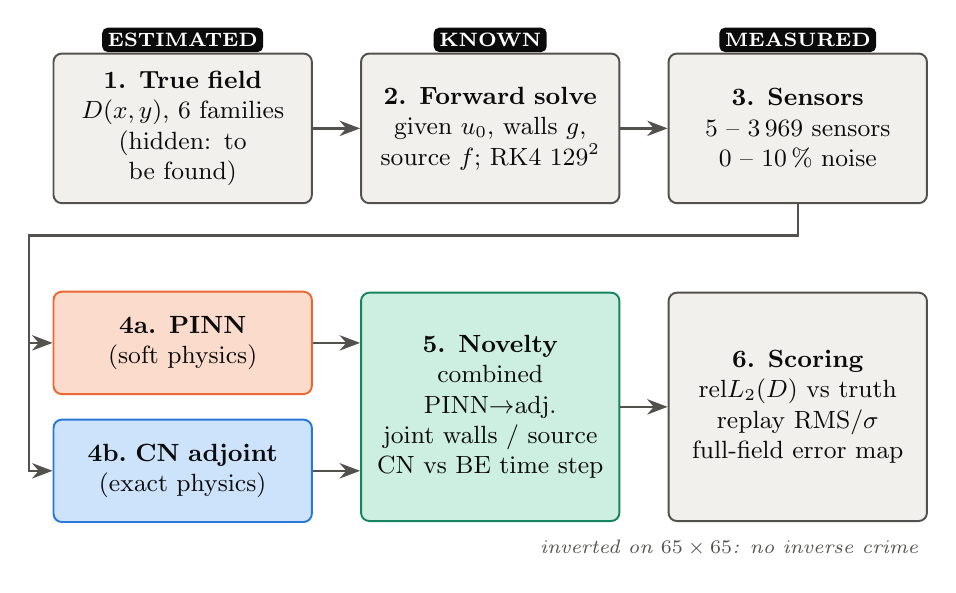
\begin{tikzpicture}[
  node distance=5mm and 6mm,
  box/.style={draw=ink2, line width=0.7pt, rounded corners=3pt, fill=neut, align=center,
              text width=#1, inner sep=4pt, font=\small\color{ink}, minimum height=19mm},
  box/.default=30mm,
  tag/.style={font=\scriptsize\bfseries\color{white}, fill=#1, rounded corners=2pt, inner sep=2pt},
  arr/.style={-{Stealth[length=2.6mm]}, line width=0.9pt, draw=ink2}]

% ---- row 1: making the data
\node[box] (truth) {{\bfseries 1. True field}\\$D(x,y)$, 6 families\\(hidden: to be found)};
\node[box, right=of truth] (fwd) {{\bfseries 2. Forward solve}\\given $u_0$, walls $g$,\\source $f$; RK4 $129^2$};
\node[box, right=of fwd] (sens) {{\bfseries 3. Sensors}\\5 -- 3\,969 sensors\\0 -- 10\,\% noise};
\node[tag=ink, anchor=south] at (truth.north) {ESTIMATED};
\node[tag=ink, anchor=south] at (fwd.north) {KNOWN};
\node[tag=ink, anchor=south] at (sens.north) {MEASURED};
\draw[arr] (truth) -- (fwd);
\draw[arr] (fwd) -- (sens);

% ---- row 2: inverting the same readings
\node[box=30mm, fill=pinnl, draw=pinn, minimum height=13mm, below=11mm of truth.south west, anchor=north west] (pinn)
  {{\bfseries 4a. PINN}\\(soft physics)};
\node[box=30mm, fill=adjl, draw=adj, minimum height=13mm, below=3mm of pinn] (adj)
  {{\bfseries 4b.\ CN\ adjoint}\\(exact physics)};
\node[box=30mm, fill=jointl, draw=joint, right=of $(pinn.east)!0.5!(adj.east)$, minimum height=29mm] (comb)
  {{\bfseries 5. Novelty}\\combined PINN$\to$adj.\\joint walls / source\\CN vs BE time step};
\node[box=30mm, right=of comb, minimum height=29mm] (score) {{\bfseries 6. Scoring}\\rel$L_2(D)$ vs truth\\replay RMS$/\sigma$\\full-field error map};

\draw[arr] (sens.south) -- ++(0,-4mm) -| ([xshift=-3mm]pinn.west) -- (pinn.west);
\draw[arr] ([xshift=-3mm]pinn.west) |- (adj.west);
\draw[arr] (pinn.east) -- (comb.west |- pinn.east);
\draw[arr] (adj.east) -- (comb.west |- adj.east);
\draw[arr] (comb) -- (score);
\node[font=\scriptsize\itshape\color{ink2}, anchor=north east] at ([yshift=-1mm]score.south east)
  {inverted on $65\times65$: no inverse crime};
\end{tikzpicture}
\end{document}
